\documentclass{beamer}
\usepackage[utf8]{inputenc}
\usepackage[T2A]{fontenc}
\usepackage[russian]{babel}
\setbeamercolor{normal text}{fg=white}
\usepackage{graphicx}
\usepackage{tikz} % Для затемнения фона титульного слайда

% Информация о презентации
\title{\textbf{История ОГУ им. Тургенева: \\
От педагогического института к современному университету.}}
\author{}
\date{}

% Настройка темы
\usetheme{Copenhagen}
\usecolortheme{orchid}

% Глобальный фон для всех слайдов, кроме титульника
\setbeamertemplate{background canvas}{%
    
\includegraphics[width=\paperwidth,height=\paperheight]{мой фон в латех.jpg}%
}

\begin{document}

% Титульный слайд с затемнённым темным фоном
{
\setbeamercolor{title}{bg=}     % Убираем фон заголовка титула
\setbeamercolor{frametitle}{bg=} % Убираем фон заголовка слайда (если появляется)
\usebackgroundtemplate{%
    \begin{tikzpicture}[remember picture,overlay]
        \node[at=(current page.center),inner sep=0]{%
            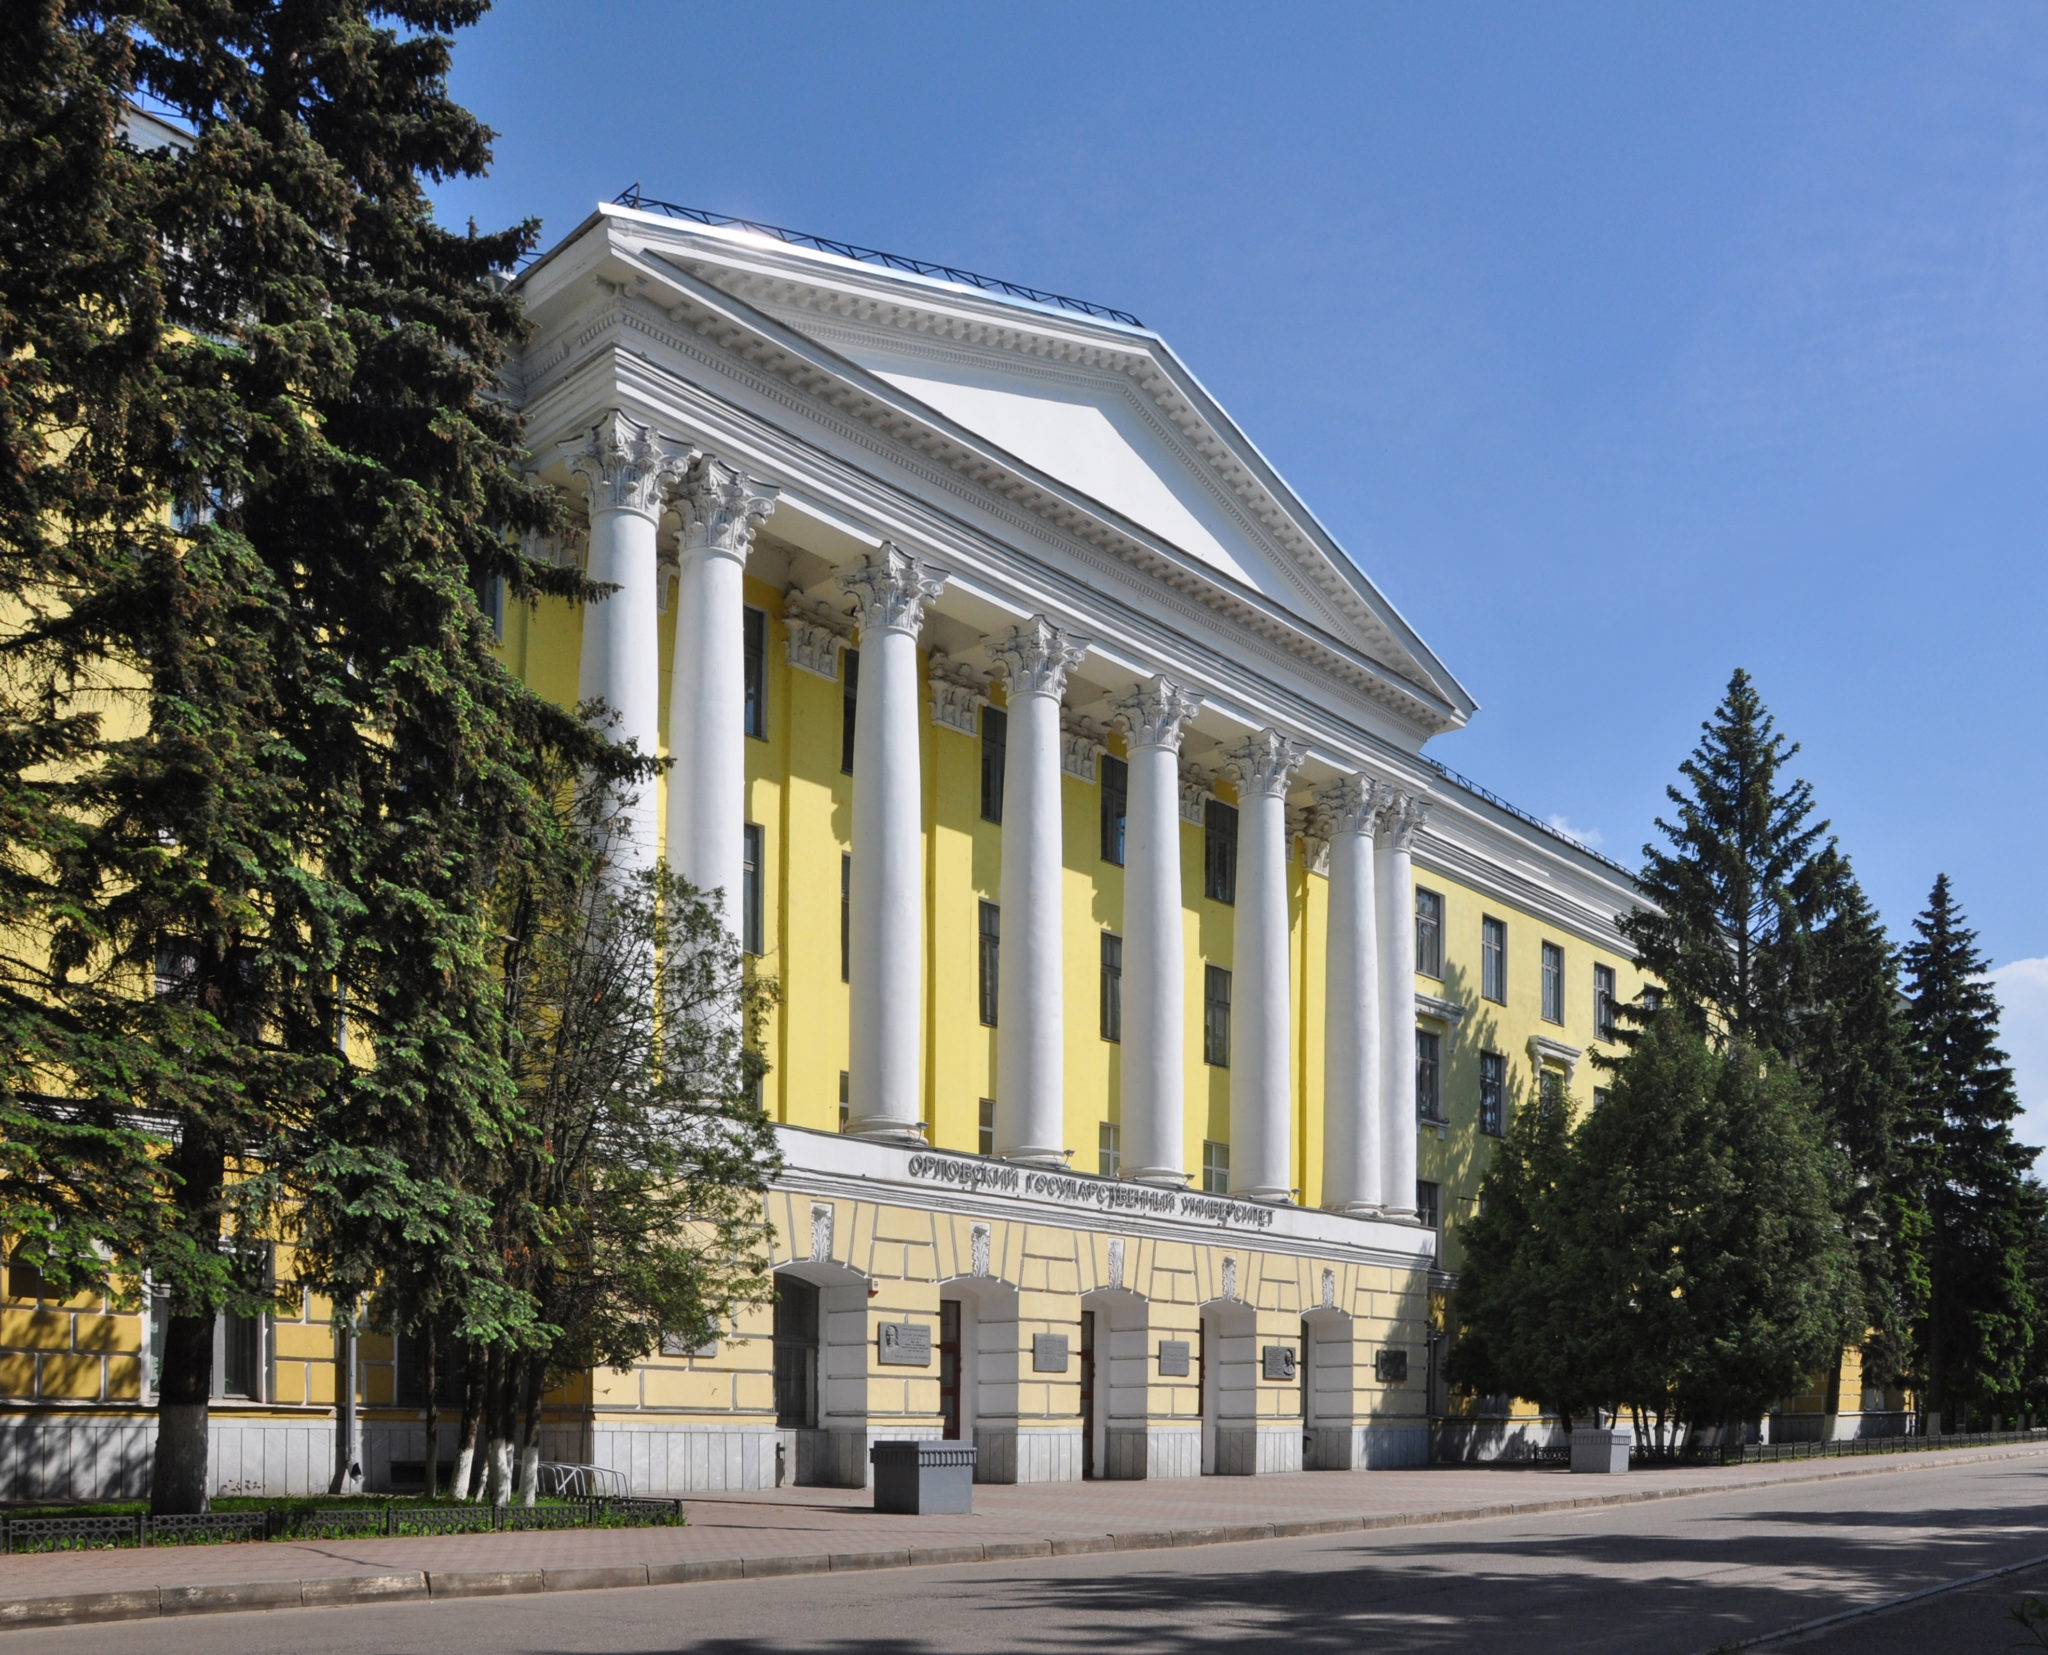
\includegraphics[width=\paperwidth,height=\paperheight]{фон на 1 слайд.jpg}%
        };
        \fill[black,opacity=0.45] (current page.south west) rectangle (current page.north east);
    \end{tikzpicture}
}
\begin{frame}[plain]
\titlepage
\end{frame}
}

% 2. Слайд с заголовком и содержимым
\begin{frame}
\frametitle{\textbf{Введение}}

\begin{columns}[T] % Выравнивание по верхнему краю
  \begin{column}{0.5\textwidth}
    {\Large
    \textbf{Сегодня мы рассмотрим:}

    \vspace{0.5em}


    \begin{itemize}
      \item Историю появления факультета
      \item Познакомимся с преподавателями 
      \item Узнаем некоторые интересные факты
    \end{itemize}
    }
  \end{column}

  \begin{column}{0.5\textwidth}
    \centering
    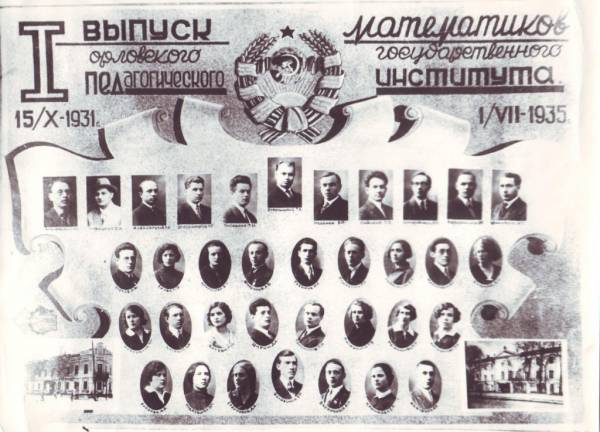
\includegraphics[width=0.9\textwidth]{1 выпуск.jpg}
    \vspace{1em}

    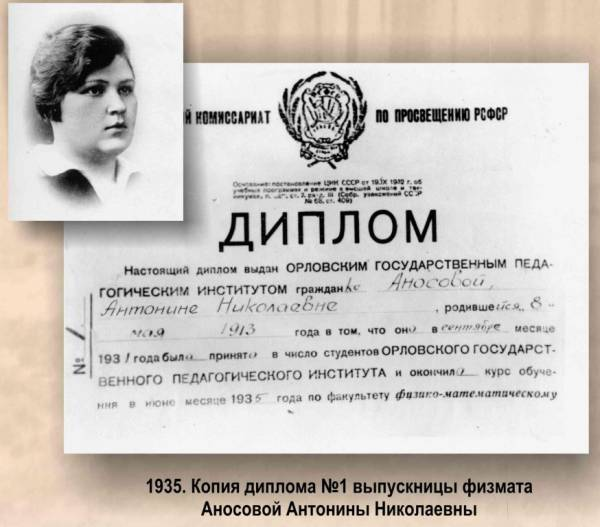
\includegraphics[width=0.75\textwidth]{1 диплом.jpg}
  \end{column}
\end{columns}
\end{frame}

% 3. Слайд с изображением и текстом
\begin{frame}
\frametitle{Наш факультет}

\begin{columns}
  \begin{column}{0.5\textwidth}
    \centering
    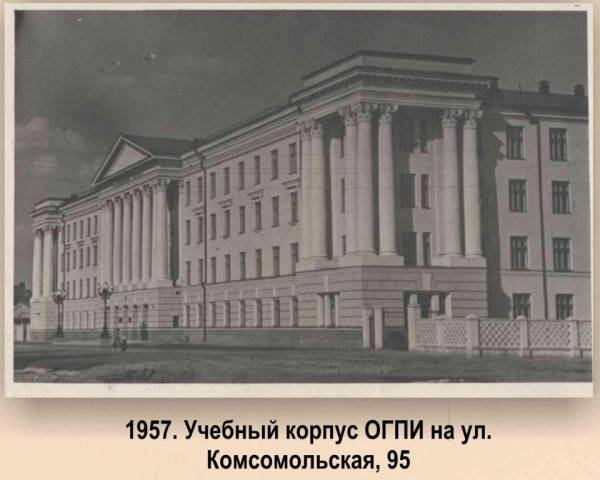
\includegraphics[width=0.99\textwidth]{фото вуза 2 слайд.jpg}
    \textit{}
  \end{column}
  \begin{column}{0.5\textwidth}
    \large В 1957 году 30 июля было сдано в эксплуатацию новое здание педагогического института. Физико-математический факультет занял 4-й этаж.
  \end{column}
\end{columns}
\end{frame}

% 4. Слайд с двумя изображениями и текстом
\begin{frame}
\frametitle{Наши ректоры}

\begin{columns}
  \begin{column}{0.45\textwidth}
    \centering
    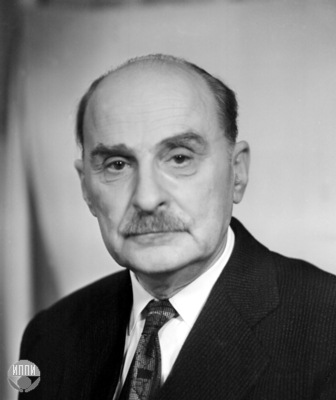
\includegraphics[width=0.8\textwidth]{Konrad_Nikolai.jpg}
    \textit{Николай Иосифович Кондрад, Первый ректор}
  \end{column}
  \begin{column}{0.45\textwidth}
    \centering
    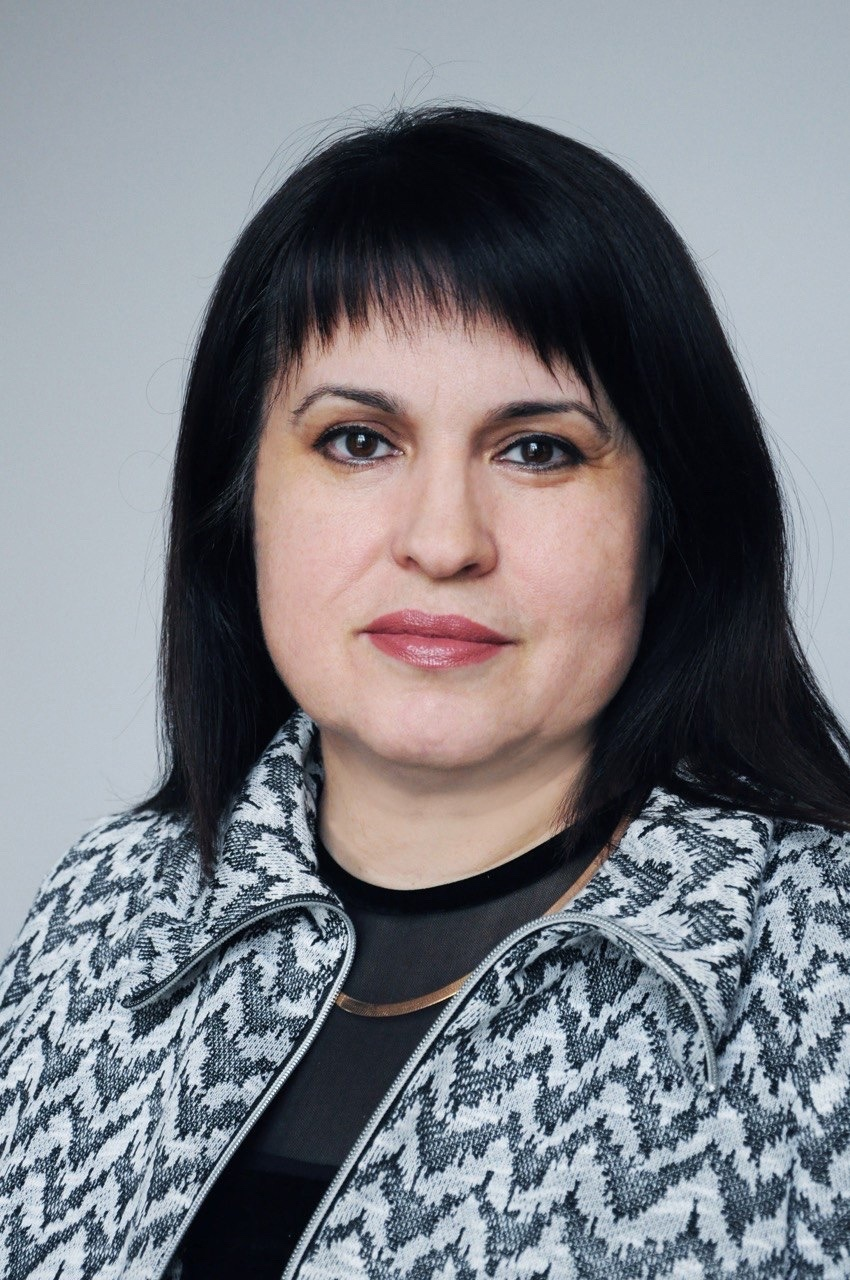
\includegraphics[width=0.8\textwidth]{Zomiteva.jpg}
    \textit{Нынешний ректор}
  \end{column}
\end{columns}

\end{frame}

% Слайд с таблицей
\begin{frame}
\frametitle{Хронология событий}

\centering
\setlength{\tabcolsep}{10pt} % Отступы между столбцами
\renewcommand{\arraystretch}{1.3} % Высота строк

\begin{tabular}{|p{2.5cm}|p{7cm}|}
\hline
\textbf{\hspace{0.7cm}Дата} & \textbf{Событие} \\
\hline
\centering 1931 год & Образование физико-математического факультета.  \\
\hline
\centering 1932 год & Физико-технический факультет был реорганизован в физико-математический. \\
\hline
\centering 1932 год & Физико-технический факультет реорганизуют в физико-математический. \\
\hline
\centering 1957 год & Вступает в строй новое учебное здание по улице Комсомольская, 95. \\
\hline
\centering 1972 год &  Для Орловского государственного педагогического института учреждают именную стипендию имени И. С. Тургенева.  \\
\hline
\centering 1992 год & Восстанавливают заочное отделение на физико-математическом факультете. \\
\hline
\end{tabular}

\end{frame}

% 6. Заключительный слайд
\begin{frame}
\centering
\Huge \textbf{Спасибо за внимание!}

\vspace{1cm}

\end{frame}

\end{document}
